\documentclass[a4paper,12pt]{article}
\usepackage[ngerman]{babel}
\usepackage[T1]{fontenc}
\usepackage[utf8]{inputenc}
\usepackage{lmodern}
\usepackage[margin=3cm]{geometry}
\usepackage{setspace}
\usepackage{amsmath, amssymb}
\usepackage{graphicx}
\usepackage{caption}
\usepackage{subcaption}
\usepackage[colorlinks=true]{hyperref}
\usepackage[hang,flushmargin]{footmisc}
\usepackage{csquotes}
\usepackage{biblatex}
\usepackage{fancyhdr}
\usepackage{tocbibind}
\usepackage{float}
\usepackage{booktabs}


\usepackage[backend=bibtex]{biblatex}
\usepackage[babel,german=quotes]{csquotes}

\addbibresource{quellen.bib}

\hypersetup{
    colorlinks=false,
    pdfborder={0 0 0}
}

\title{Bachelorarbeit}
\author{Tom Becke}
\date{\today}
\setlength{\parindent}{0pt}

\begin{document}

\doublespacing

\maketitle

\begin{center}
    {\LARGE \textbf{Leistungs- und Renderzeitvergleich von React Native und Flutter: Eine Analyse der Performance moderner Cross-Plattform-Frameworks}}
\end{center}

\newpage

\tableofcontents

\newpage

\input{Einführung}
\section{Methoden der Softwareentwicklung}
Die Softwareentwicklung lässt sich in verschiedene Kategorien einteilen. Die Backend-Entwicklung befasst sich mit der Serverseite einer Anwendung. Es werden Anfragen an das Backend geschickt, welches die Anfragen verarbeitet und eine Antwort zurückliefert. Datenbanken, Microservices und weitere diverse Funktionalitäten werden im Backend umgesetzt und sind dadurch strikt vom Frontend getrennt.

\vspace{0.5cm}

Das Frontend beschreibt den Teil einer Anwendung, der auf dem Endgerät läuft und dafür zuständig ist, Eingaben zu verwalten oder Daten vom Backend darzustellen. Die Benutzeroberfläche wird durch verschiedene Elemente repräsentiert, die der Anzeige von Daten dienen oder dem Benutzer die Möglichkeit bieten, mit der Schnittstelle zu interagieren. In dieser Arbeit steht das Frontend im Vordergrund, da der Fokus der behandelten Frameworks in diesem Bereich liegt.

\vspace{0.5cm}

\subsection{Codeebenen}
\subsubsection{Maschinencode}

Die tiefste Ebene der Programmiersprachen bilden die Maschinensprachen oder Assembler-Sprachen ab. Diese Sprachen werden direkt auf dem Prozessor des Zielsystems interpretiert und ausgeführt. Da verschiedene Prozessoren unterschiedliche Befehle verarbeiten können, muss der Code für das jeweilige Zielsystem ausgelegt sein. Assembler-Sprachen sind also plattformspezifisch und erfordern eine genaue Abstimmung auf das Endgerät.

\vspace{0.5cm}

\subsubsection{Bytecode}

Einige Programmiersprachen verwenden Bytecode, um den geschriebenen Quellcode in eine Zwischensprache zu übersetzen. Dies ermöglicht es, den Code auf verschiedenen Endgeräten laufen zu lassen, ohne ihn anpassen zu müssen. Sprachen wie Java nutzen Bytecode und benötigen eine virtuelle Maschine (z.B.: JVM), die den Zwischencode zur Laufzeit in Maschinensprache für das jeweilige Zielsystem übersetzt.

\vspace{0.5cm}

\subsection{Native Entwicklung - iOS und Android}

Möchte man auf bestimmte Funktionen eines Endgeräts zugreifen, ist eine native Entwicklung erforderlich. Bei Android-Geräten wird häufig Kotlin verwendet, während iOS-Apps in Swift programmiert werden. Native Software greift direkt auf das Betriebssystem zu und muss daher plattformspezifisch sein. Kotlin und Swift bieten leistungsstarke Möglichkeiten, um direkt auf die Hardware und nativen Funktionen der Geräte zuzugreifen.

\vspace{0.5cm}

\subsection{Webbasierte Software}

Die verbreiteste Möglichkeit, ein Frontend zu entwickeln, ist die webbasierte Programmierung. Mit HTML (Hyper Text Markup Language) werden Komponenten entwickelt, die von einem Webbrowser interpretiert und dargestellt werden. HTML implementiert jedoch keine Logik. Um die Benutzeroberfläche mit Funktionen auszustatten, wird JavaScript genutzt, das dynamisch zur Laufzeit kompiliert wird. Um die Benutzeroberfläche zu manipulieren, wird das DOM (Document Object Model) verwendet, das eine Schnittstelle zwischen HTML und JavaScript darstellt.

\vspace{0.5cm}

Frameworks wie Angular, React oder Vue.js erleichtern die Entwicklung von Webanwendungen durch strukturierte Ansätze und die Möglichkeit, wiederverwendbare Komponenten zu erstellen. Diese Frameworks nutzen oft ein virtuelles DOM, das für eine effiziente Aktualisierung und Verwaltung der Benutzeroberfläche sorgt. Das virtuelle DOM ist eine Abstraktion des tatsächlichen DOMs und ermöglicht es, Änderungen an der Benutzeroberfläche schneller und effizienter zu verarbeiten. Statt direkt das reale DOM zu manipulieren, wird eine Kopie des DOMs im Speicher gehalten. Wenn sich der Zustand der Anwendung ändert, wird zunächst das virtuelle DOM aktualisiert. Anschließend wird der Unterschied zwischen dem aktuellen und dem vorherigen Zustand des virtuellen DOMs (Reconciliation) berechnet und nur die minimal notwendigen Änderungen auf das echte DOM angewendet. Dies sorgt für eine optimierte Performance und vermeidet unnötige und teure DOM-Manipulationen.

\subsubsection{WebAssembly (Wasm)}
WebAssembly (Wasm) wurde entwickelt, um eine effiziente, portierbare und sichere Laufzeitumgebung bereitzustellen, die JavaScript ergänzt. Es bietet die Möglichkeit, leistungskritische Anwendungen im Browser auszuführen. WebAssembly basiert auf Bytecode, der in einer binären Form vorliegt und direkt vom Browser interpretiert wird, was eine schnellere Ausführung als bei der Interpretation von JavaScript-Quellcode ermöglicht. Es ist möglich, WebAssembly von Hand zu programmieren, aber meistens wird eine Sprache zu WebAssembly kompiliert, hierzu zählen C, C++, Rust, Go und Dart in ausgewählten Fällen. Durch die Umwandlung in eine binäre Befehlsform wird eine Performance erreicht, die nahezu der nativen Geschwindigkeit entspricht. WebAssembly zeigt in bestimmten Szenarien eine bis zu 17,24 \% schnellere Performance. Darüber hinaus ist auch die Energieeffizienz deutlich besser, mit einer Einsparung von ca. 30,69 \% im Vergleich zu JavaScript 
\cite{WebAssemblyVsJavaScript}

\subsubsection*{Vorteile webbasierter Software}

- Funktioniert in jedem Webbrowser auf jedem Endgerät \\
- Breit gefächertes Expertenwissen \\
- Viele Frameworks und Bibliotheken erleichtern die Arbeit

\subsubsection*{Nachteile webbasierter Software}

- Kompilierung nur durch den Webbrowser \\
- Fehlende Möglichkeit, spezifische Funktionen des Endgeräts zu nutzen \\
- Geringere Performance \\
- Fehlende Sicherheit durch sichtbaren Code

\subsection{Cross-Plattform Entwicklung}

Cross-Plattform-Entwicklung ermöglicht es, einen Quellcode zu schreiben, der auf verschiedenen Endgeräten läuft. Dies spart Zeit und Kosten, da nicht für jedes Betriebssystem ein separater Code entwickelt werden muss. Frameworks wie React Native und Flutter erlauben es, den Quellcode in die native Sprache des Zielsystems zu übersetzen, was die Leistung verbessert und den Zugriff auf native Funktionen ermöglicht.

\subsubsection*{Vorteile der Cross-Plattform-Entwicklung}

- Zeitersparnis \\
- Wiederverwendbarkeit des Codes \\
- Ähnliches Design wie bei nativen Komponenten \\
- Leichtere Instandhaltung und Einbindung neuer Updates \\

\subsubsection*{Nachteile der Cross-Plattform-Entwicklung}

- Vereinzelt fehlende native Funktionen \\
- Größere kompilierte Apps auf den Endgeräten \\
- Potenzielle Einbußen in der Leistung

Aufgrund der steigenden Popularität von Cross-Plattform-Frameworks und der Vielzahl an Vorteilen werden im Folgenden zwei der bekanntesten Frameworks, Flutter und React Native, näher betrachtet.

\section{React Native im Detail}
React Native wurde von Meta Platforms Inc. (ehemals Facebook) entwickelt und erschien im Jahr 2015. Die Handhabung von React Native ist sehr ähnlich zu der von klassischem React für die webbasierte Softwareentwicklung. Der komponentenbasierte Ansatz beim Entwickeln und die Möglichkeit, JavaScript oder TypeScript zu verwenden, bieten erfahrenen Entwicklern eine vertraute Umgebung. Durch den Einsatz von JavaScript gibt es eine große Auswahl an Bibliotheken und eine große Community.

\vspace{0.5cm}

React Native verwendet weder den DOM noch einen virtuellen DOM. Stattdessen werden React-Komponenten in native UI-Komponenten der jeweiligen Plattform übersetzt (z. B. UIView auf iOS oder View auf Android). Dies ermöglicht eine plattformnative Darstellung der Benutzeroberfläche, während die zugrunde liegende Logik weiterhin in JavaScript implementiert wird.

Der JavaScript-Code wird nicht direkt in nativen Code kompiliert, sondern in einer JavaScript-Engine (z. B. Hermes, JavaScriptCore oder V8) ausgeführt. Die Kommunikation zwischen der JavaScript-Logik und der nativen Plattform erfolgt über eine sogenannte Bridge.

\vspace{0.5cm}

Die Bridge dient als bidirektionale Verbindung, über die Nachrichten zwischen JavaScript und der nativen Ebene ausgetauscht werden. Diese Nachrichten definieren, welche Aktionen ausgeführt werden sollen, und liefern die dazugehörigen Anweisungen. Ein typisches Beispiel ist das Rendern einer View: Die JavaScript-Seite sendet eine Nachricht an die native Seite, die daraufhin die entsprechende UI-Komponente erstellt und darstellt.

\vspace{0.5cm}

\begin{figure}[H]
    \centering
    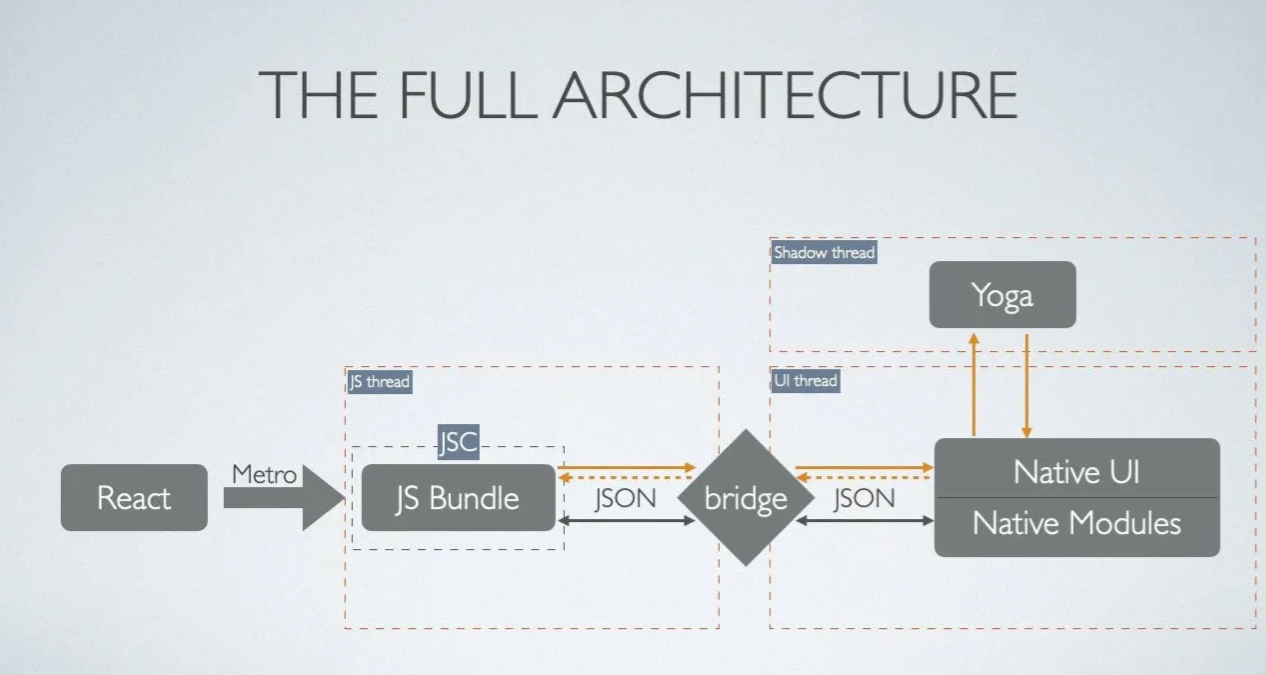
\includegraphics[width=0.9\linewidth]{images/reactnative-bridge.png}
    \caption{Visuelle Darstellung der Brücke \cite{ReactNativeBridge}}
\end{figure}

Umgekehrt funktioniert die Kommunikation genauso: Wenn in der View eine Eingabe erfolgt, wird über die Bridge eine Nachricht an die JavaScript-Seite gesendet. Diese Informationen werden asynchron übertragen und von der Bridge zwischen den beiden Parteien verwaltet. Die Asynchronität trägt dazu bei, dass Views flüssig dargestellt werden können. Ziel ist es, eine Bildwiederholrate von ca. 60 Bildern pro Sekunde zu erreichen. Die tatsächliche Leistung hängt jedoch von mehreren Faktoren ab, unter anderem von der Komplexität des Layouts und der Menge der Nachrichten, die über die Bridge gesendet werden.

\vspace{0.5cm}

Eine zu große Anzahl von Nachrichten über die Bridge kann zu einem so genannten „Bridge-Stau“ führen, der die Performance beeinträchtigt. Um dies zu minimieren, wird häufig die JavaScript-Engine \textit{Hermes} verwendet. Hermes kompiliert JavaScript in Bytecode, der direkt auf dem Endgerät ausgeführt wird, was die Laufzeit- und Startleistung verbessert. Wenn Hermes deaktiviert ist, verwendet React Native \textit{JavaScriptCore}, die Standard-JavaScript-Engine von iOS. JavaScriptCore hat jedoch den Nachteil, dass es keine \textit{JIT}-Kompilierung auf iOS-Geräten unterstützt, was die Performance beeinträchtigen kann.

\vspace{0.5cm}

Ein weiterer wichtiger Bestandteil des Kompilierungs- und Bauprozesses ist der \textit{Metro-Bundler}, der die JavaScript-Dateien bündelt und für die Ausführung auf dem jeweiligen Endgerät vorbereitet.

\vspace{0.5cm}

React Native verwendet native Build-Systeme, um die Applikationen für die jeweiligen Endgeräte zu bauen. Dabei nutzt Android das Build-System \textit{Gradle}, während iOS auf \textit{Xcode} zurückgreift. Der Metro-Bundler bündelt die JavaScript-Dateien zu einer einzigen Datei, die zur Laufzeit von einer JavaScript-Engine (z. B. Hermes oder JavaScriptCore) interpretiert wird. Diese gebündelten Dateien werden zusammen mit den nativen Komponenten der App in eine \textit{APK} für Android oder eine \textit{IPA} für iOS verpackt und signiert.

\vspace{0.5cm}

React Native bietet von Haus aus keine Möglichkeit, Anwendungen für das Web zu erstellen. Hierfür kann eine zusätzliche Bibliothek genutzt werden, die die Möglichkeit bietet, den React-Quellcode für den Browser zu nutzen. Diese Bibliothek übersetzt React-Native-Komponenten in standardmäßige React-DOM-Komponenten, sodass sie in Webbrowsern lauffähig sind. Der Build-Prozess ist hierbei identisch zu der Kompilierung von klassischem React-Code.

Ein Auszug der Plattformen, für die React Native verwendet werden kann:
\url{https://reactnative.dev/docs/out-of-tree-platforms}
\section{Flutter im Detail}
Flutter ist ein von Google entwickeltes Cross-Plattform-Framework. Es wurde erstmalig 2017 als Open-Source-Software veröffentlicht. Flutter nutzt eine eigene Architektur beim Aufbau der Software. Es werden Widgets genutzt, um Darstellung, Logik und Interaktionen innerhalb eines Objektes zu vereinen. Vorgefertigte Komponenten erleichtern den Entwicklungsprozess, indem sie häufig verwendete Elemente wie Schaltflächen, Texte, Checkboxen usw. vordefinieren. Diese Widgets orientieren sich in ihrem Design an den Richtlinien der jeweiligen Zielsysteme, wie z. B. Material Design für Android oder Cupertino Design für iOS. Flutter nutzt als Programmiersprache \textit{Dart}, die von Google entwickelt wurde und eine moderne Alternative zu JavaScript darstellt.

\vspace{0.5cm}

Flutter verfolgt bei der Kompilierung einen anderen Ansatz als React Native, um eine bestmögliche Performance zu erreichen. Der Dart-Code wird zu nativem Maschinencode kompiliert (Ahead-of-Time), anstatt die UI-Komponenten in native Komponenten umzuwandeln. Stattdessen verwendet Flutter die Skia-Rendering-Engine, um die Benutzeroberfläche direkt zu rendern. Dieser Ansatz ermöglicht eine konsistente Leistung und gibt Flutter die volle Kontrolle darüber, wie Komponenten dargestellt und miteinander interagieren. Während der Entwicklung kommt die Dart Virtual Machine (DVM) zum Einsatz, die Funktionen wie Hot Reload unterstützt. Im Produktionsmodus wird jedoch ausschließlich nativ kompilierter Code verwendet, was zu einer flüssigen und leistungsstarken Benutzererfahrung führt.

\vspace{0.5cm}

Der kompilierte Code für die Grafik-Rendering-Engine wird bei Android mit dem NDK (\textit{Native Development Kit}) und bei iOS mit LLVM kompiliert. Während der Entwicklung verwendet Flutter die Dart VM mit \textit{Just-in-Time} (JIT) Kompilierung, was Funktionen wie \textit{Hot Reload} ermöglicht. Dieses Feature erlaubt es, Änderungen im Quellcode nahezu sofort in der Entwicklungsumgebung sichtbar zu machen, ohne die Anwendung neu zu starten. Die AOT-Kompilierung erstellt eine APK (für Android) oder IPA (für iOS), welche für die Veröffentlichung und Installation auf den jeweiligen Endgeräten genutzt werden kann.

\vspace{0.5cm}

\textit{Dart Web} ermöglicht die Kompilierung für das Web. Der Dart-Quellcode wird wahlweise in JavaScript oder WebAssembly übersetzt, wodurch er im Browser ausgeführt werden kann. Für das Darstellung stehen zwei Ansätze zur Verfügung: der HTML-Renderer und das CanvasKit. Der HTML-Renderer setzt auf JavaScript, um HTML- und CSS-Elemente zu generieren, während das CanvasKit den Dart-Code in WebAssembly kompiliert, um eine GPU-beschleunigte Darstellung über WebGL zu ermöglichen. Beide Optionen bieten Entwicklern Flexibilität, je nach Anforderungen ihrer Anwendung.

\vspace{0.5cm}

Die \textit{Dart SDK} stellt die nötigen Command-line-Tools zur Verfügung, um die Entwicklung zu erleichtern. Dazu gehört unter anderem der \textit{Linter}, der \textit{Dart pub Package Manager} und viele weitere Funktionen.

\vspace{0.5cm}

Der Zugriff auf native Funktionen des Endgeräts in Flutter erfolgt über \textit{Method Channels}. Flutter selbst ist plattformunabhängig und bietet daher keinen direkten Zugriff auf system- oder gerätespezifische APIs. Um dennoch auf native Funktionen wie die Kamera oder Galerie zugreifen zu können, wird ein sogenannter \textit{Method Channel} genutzt.

\vspace{0.5cm}

Ein \textit{Method Channel} ermöglicht die Kommunikation zwischen dem Dart-Code von Flutter und dem nativen Code der jeweiligen Plattform (Android oder iOS). Dazu muss ein Kanal erstellt werden, der als Brücke zwischen dem Flutter-Frontend und den API-Funktionen des Endgeräts fungiert. Der Dart-Code sendet Anfragen über diesen Kanal und der native Code antwortet, indem er die entsprechenden Betriebssystemfunktionen aufruft.

\vspace{0.5cm}

Beispielsweise wird bei der Auswahl eines Bildes über den \textit{Method Channel} eine Anfrage an das Endgerät gesendet, die die native Funktion zum Öffnen der Galerie aufruft. Nach der Auswahl eines Bildes wird dieses zurückgesendet und kann im Flutter-Quellcode verwaltet und angezeigt werden.
\section{Anforderungsanalyse}

Diese Arbeit verfolgt das Ziel, einen Vergleich der Leistung von React Native und Flutter durchzuführen. Der Vergleich wird durch verschiedene Benchmarks getätigt, welche eine konstante und vergleichbare Bewertung der Frameworks ermöglichen. Es werden praxisnahe Anforderungen an die Frameworks gestellt, welche die Darstellung von Elementen und die Nutzung der nativen Funktionen auf verschiedenen Endgeräten testen. Die fundamentale Forschungsfrage der Arbeit lautet:

\textit{Welche messbaren Unterschiede in der Darstellungsleistung ergeben sich im Vergleich zwischen Flutter und React Native in modernen Cross-Plattform-Anwendungen?}

Daraus lassen sich folgende Unterfragen ableiten:

\begin{enumerate}
    \item Wie unterscheiden sich React Native und Flutter in Render- und Rechenleistung bei typischen Entwicklungsaufgaben?
    \item Gibt es Unterschiede der Leistung auf verschiedenen Endgeräten?
    \item Welches Framework ist für die alltägliche Praxis im Hinblick auf die Leistung attraktiver?
\end{enumerate}

\subsection{Auswahl der Benchmarks}

Es wird ein Benchmark genutzt, welcher die Darstellung von verschiedenen Elementen mithilfe von Animationen beinhaltet. Es wurden Tests gewählt, welche die Darstellung von Elementen, komplexeren Animationen, die Rechenleistung, die Zustandsverwaltung und die Funktion von nativen Methoden überprüfen. Die Tests werden mit einem Chromium-basierten Browser und einem emulierten Android-Gerät durchgeführt. Zum Schluss werden die Messwerte jedes Benchmarks in einem Diagramm dargestellt, um einen optischen Vergleich der Resultate zu erhalten.

\subsubsection*{Würfel}

Es wird eine Anzahl an Würfeln auf dem Endgerät dargestellt. Diese Würfel sind in einem durchgehenden Farbwechsel und sie rotieren um ihre eigene Achse. Ebenfalls bewegen sie sich stetig zu zufälligen Positionen innerhalb des Bildschirms. Es gibt zwei verschiedene Durchführungen, eine mit 100 dargestellten Würfeln und eine mit 1000 Würfeln. Es wird festgehalten, wie viele Frames pro Sekunde berechnet werden konnten. Die Messung erfolgt im Browser über den Chromium Performance Monitor innerhalb der DevTools. Dort lässt sich die Zeit ablesen, die es gebraucht hat, um einen einzelnen Frame darzustellen, wodurch sich die Frames pro Sekunde (FPS) ausrechnen lassen. Auf dem Android-Gerät gibt es einen eingebauten Performance Monitor, welcher mir direkt die FPS anzeigt.

\subsubsection*{Speicher}

Ein weiterer Praxisfall ist das Speichern von großen Daten auf den jeweiligen Plattformen. Hierbei wird simuliert, dass eine große Menge an Daten im JSON-Format gespeichert wird, daraufhin geladen wird und in ein Objekt geparsed wird. Es wird hierbei die Zeitmessung gestartet, sobald das Speichern beginnt und endet mit dem erfolgreichen Parsen der Daten in ein Objekt.

\subsubsection*{Sieb des Eratosthenes}

Die Leistung der kompilierten Sprache wird durch das Sieb des Eratosthenes geprüft. Hierbei wird berechnet, wie viele Primzahlen sich bis zur gegebenen Zahl n befinden. Dieser Benchmark erfordert einiges an Rechenleistung und dient daher als guter Richtwert für die reine rechnerische Leistung der Anwendung. Die Messung umschließt die Dauer der Berechnung der Menge an Zahlen.

\subsubsection*{State Management}

Für viele Entwickler ist das State Management von großer Bedeutung in der Entwicklung einer Anwendung, weil darüber verschiedene Zustände, die in einer Anwendung auftreten, verwaltet werden. In diesem Test wird einem State, welcher eine Liste aus Strings beinhaltet, eine große Anzahl an Objekten hinzugefügt, welche daraufhin angezeigt werden und danach wieder aus dem State entfernt werden, damit sie verschwinden. Gemessen wird die Zeit zwischen dem Zeitpunkt, zu dem die Elemente dem Zustand hinzugefügt werden, und dem Zeitpunkt, zu dem sie aus dem Zustand entfernt werden.

\subsection{Vergleichbarkeit der Benchmarks}

Die Benchmarks sind darauf ausgelegt, vergleichbare Messwerte zu produzieren. Die Bedingungen und die Umgebung sind für beide plattformübergreifenden Frameworks identisch. Über einen zeitlichen Verlauf oder über die Anzahl der Durchführungen lassen sich die Messwerte eines einzelnen Durchlaufs chronologisch ordnen. Die Messungen werden insgesamt 3 Mal durchgeführt, wodurch bei jeder Durchführung eine festgelegte Anzahl an Messwerten produziert wird. Es wird festgehalten, wie viele Bilder pro Sekunde dargestellt werden können oder wie lange es dauert, bis eine Darstellung fertig gerendert ist. 


\section{Implementierung}
\subsection{Expo}

Bei der Entwicklung der Benchmarks in React Native wurde Expo genutzt, um die Implementierung zu erleichtern. Expo ist ein Framework, welches den Umgang mit React Native verbessert. Es liefert Tools fürs Debugging, erleichtert das Bauen und Starten von nativen Apps und bietet eine große Auswahl an Bibliotheken.

\subsection{Grundlegendes}

Die Implementierung ist darauf ausgelegt, auf beiden Frameworks nahezu identisch zu sein. Es werden Packages genutzt, welche von den Frameworks direkt zur Verfügung gestellt wurden oder welche von den Entwicklern empfohlen wurden. Sowohl die React Native App als auch die Flutter App wurden auf dem Emulator via APK Export installiert, um jeglichen Leistungsverlust durch den Entwicklermodus zu vermeiden. Im Web werden die Anwendungen als exportiertes Kompilat getestet, damit keine Entwicklerumgebung das Ergebnis verfälschen könnte.

\subsection{Testumgebung}
\begin{table}[h!]
\centering
\begin{tabular}{|c|c|c|}
\hline
\textbf{System} & \textbf{Version} & \textbf{Besonderheiten} \\
\hline
Windows & Chromium basierter Browser & Blink / V8 \\
\hline
Android Emulator & Pixel 8 mit API 35 & 4 CPU Kerne, 4 GB RAM \\
\hline
\end{tabular}
\end{table}

\subsection{Würfel}

\subsection*{React Native}

Es wurde eine View über den gesamten Anzeigebereich gestaltet. In dieser View wird eine Anzahl an Würfel-Komponenten gerendert. Ein Array mit einer Größe von der festgelegten Anzahl an darzustellenden Würfeln legt die Anzahl der dargestellten Elemente fest. Die Darstellung eines einzelnen Würfels wird durch eine separate Komponente realisiert. 

Eine \texttt{Animated View}, bei der die Argumente Position, Rotation und Hintergrundfarbe ständig verändert werden, umfasst eine View, in der sich ein Text mit dem Unicode eines Würfels befindet, der dauerhaft die Farbe wechselt. Alle 2 Sekunden wird die Rotation des Würfels auf den Ursprung gesetzt, sowie eine neue Zielposition bestimmt und eine neue Farbe festgelegt. Die Argumente Position und Rotation werden über einen \texttt{useState} verwaltet. 

In einem \texttt{useEffect} wird dafür gesorgt, dass beim Rendern der Komponente die wichtigen Funktionen aufgerufen werden. Die Bewegung des Würfels wird durch die Funktion \texttt{animatePosition} ermöglicht, welche zufällige \(x\) und \(y\) Werte bestimmt und diese durch \texttt{Animated.timing} in einem flüssigen Übergang darstellt. 

Die Rotation wird ebenfalls durch \texttt{Animated.timing} verwaltet, wobei die Rotation bei dem Wert 0 startet und bei 1 endet. Durch \texttt{rotation.interpolate} wird im späteren Verlauf des Codes festgelegt, dass der Wert 0 für \(0^\circ\) steht und 1 für \(360^\circ\). Dies sorgt für eine vollständige Rotierung um die eigene Achse in einem flüssigen Übergang. Farblich ändert sich der Würfel, indem ein Array aus den vorhandenen Farben angelegt wird und bei dem Aufruf durch das Intervall ein neuer Index bestimmt wird. Der jeweilige Farbeintrag aus dem Array wird ausgelesen und der View zugeschrieben.

\subsection*{Flutter}

Die View wird so gestaltet, dass eine festgelegte Anzahl an animierten Würfeln auf dem Bildschirm dargestellt wird. Die Anzahl der Würfel wird durch eine Liste generiert. Jeder Würfel wird durch eine Komponente realisiert, die sowohl in Farbe als auch in Position und Rotation animiert ist. 

Ein \texttt{AnimationController} steuert die Animationen der Würfel, die alle 2 Sekunden wiederholt werden. Die Würfel ändern ihre Farbe kontinuierlich, indem ein \texttt{ColorTween} verwendet wird, um zwischen Farben aus einer vordefinierten Liste von Farben zu wechseln. Die Position jedes Würfels wird zufällig bestimmt, wobei der Ausgangs- und Zielort innerhalb des Bildschirms zufällig gesetzt wird. 

Die Rotation erfolgt kontinuierlich über den Animationscontroller und befindet sich zwischen \(0^\circ\) und \(360^\circ\). Die Animation wird in einer \texttt{AnimatedBuilder}-Komponente gerendert, die sicherstellt, dass der Würfel sich sowohl in Position, Rotation als auch Farbe flüssig ändert.

\begin{figure}[H]
    \centering
    \begin{minipage}{0.49\textwidth}
        \centering
        \includegraphics[width=\linewidth]{images/code/cube_react.png}
        \caption{Codeauszug React Native}
    \end{minipage} \hfill
    \begin{minipage}{0.49\textwidth}
        \centering
        \includegraphics[width=\linewidth]{images/code/cube_flutter.png}
        \caption{Codeauszug React Native}
    \end{minipage}
\end{figure}

\subsection{Storage}

\subsection*{React Native}
Es wird ein Array von Objekten erstellt, das aus String-Attributen besteht, aus einem Attribut besteht und diese Objekte werden vom Package \texttt{faker} mit Beispielwörtern gefüllt. \texttt{Faker} erzeugt algorithmisch Beispieldaten, welche für den Test optimal sind, da sie künstlich eine große Menge an Daten abbilden. Der Async Storage wird in React Native dafür genutzt, um anhand eines Keys ein Value-Objekt zu speichern. Als Speicherort wird im Browser der Localstorage genutzt und auf dem Android-Gerät wird eine SQLite-Datenbank erzeugt. Zu Beginn des Tests wird der Async Storage komplett geleert und daraufhin wird das große Objekt unter dem Key \texttt{jsonData} gespeichert. Im nächsten Schritt wird dieses Objekt, welches als JSON-String gespeichert wurde, ausgelesen und in das ursprüngliche Objekt geparsed. Sobald das ursprüngliche Array aus den Objekten erzeugt wurde, endet die Zeitmessung und die Dauer wird ermittelt.

\subsection*{Flutter}
Hier ist die Funktionsweise des Speicherns ein wenig anders. Im Browser speichert Flutter die Daten ebenfalls im LocalStorage, jedoch auf dem Android-Gerät greift Flutter auf das Interface des Android-Gerätes namens Shared Preferences zu. Dies erlaubt ebenfalls eine Speicherung von einem Datentypen anhand eines Keys, jedoch wird keine eigenständige Datenbank generiert. 

\subsection{Sieb des Eratostehenes}

\subsection*{React Native \& Flutter}
Dieser Benchmark beginnt nach dem Starten mit der Zeitmessung. Im nächsten Schritt wird ein Timeout gesetzt, da dies dafür sorgt, dass die Berechnung nicht im Hintergrund passiert, sondern der Main Thread blockiert wird und für die Berechnung genutzt wird. Dies verhindert ein asynchrones Verhalten und vermeidet Fehler bei der Messung sowie ein langsameres Resultat bei der Berechnung. Die Berechnung besteht aus einem Algorithmus, welcher eine Liste der Länge der gegebenen Zahl \texttt{n} entspricht. Alle Felder werden vorerst mit \texttt{true} vorbelegt. Nun werden die Primzahlen ausgesiebt, wozu die Vielfachen von 2 und alle weiteren Vielfachen der kommenden Zahlen zählen. Zahlen, die keine Vielfachen sind, bleiben weiterhin als true markiert und werden in ein separates Array namens Output zusammengefasst. Daraufhin wird die Länge des Output Arrays angezeigt, um die korrekte Ausführung des Algorithmus zu verifizieren, und die Zeitmessung endet. In Bezug auf den Flutter Code lässt sich festhalten, dass dieser keinen funktionalen Unterschied zum React Native Code aufweist.

\subsection{State Management}

\subsection*{React Native}
Hier wird getestet, wie schnell die Anwendung mit einem Wechsel diverser Zustände umgehen kann. Es wird ein useState erstellt, welcher ein Array aus Strings beinhaltet. Nach dem Starten des Benchmarks wird der State mit einem Array befüllt. Daraufhin wird ein Timeout gesetzt, welcher wiederum dafür sorgt, dass der Mainthread für die Verarbeitung genutzt wird. Dieser Timeout hat eine Verzögerung von 50ms, welche durch die Funktionsweise und die Adaption des Codes von Flutter vorhanden ist. Durch den useState werden kurz alle Elemente angezeigt, nachdem sie gesetzt wurden und danach werden sie wieder aus dem State entfernt. Die Zeitmessung endet nach dem erfolgreichen Leeren des Zustandes.

\subsection*{Flutter}
Der Aufbau des Benchmarks in Flutter funktioniert nahezu identisch zu dem in React Native. Dabei ist zu beachten, dass in Flutter alle Elemente innerhalb eines StatefulWidget automatisch einen Zustand verwalten, ähnlich wie useState in React Native. Änderungen am Zustand eines StatefulWidget führen zu einem Rerendering des Widgets. Die Zeitverzögerung im Timeout ist in Flutter notwendig, da sonst das Ändern des States in den Hintergrund gerät und die Zeiterfassung schon beendet wird, während des State noch befüllt ist.

\newpage
\subsection{Auswertung der Messergebnisse}
Die erhaltenen Ergebnisse werden in einer CSV-Datei festgehalten. Aus allen drei Durchläufen wird der Durchschnittswert für jeden Messpunkt berechnet, um diesen grafisch darzustellen. Die grafische Darstellung erfolgt auf Grundlage der CSV-Dateien in R, einer Programmiersprache, die zur Visualisierung von Daten genutzt werden kann. Auf der Y-Achse des Diagramms wird der gemessene Wert, sei es die FPS (Frames per Second) oder eine gemessene Zeitspanne, abgebildet. Auf der X-Achse wird der zeitliche Verlauf oder die Nummer des Durchlaufs dargestellt. Im Diagramm wird eine rote Linie für React Native und eine blaue Linie für Flutter eingezeichnet.
\newpage
\section{Ergebnisse}
\subsection{100 Würfel Animation}
Für die beiden folgenden Tabellen gilt, dass ein höheres Ergebnis eine bessere Leistung darstellt.
\begin{figure}[H]
    \centering
    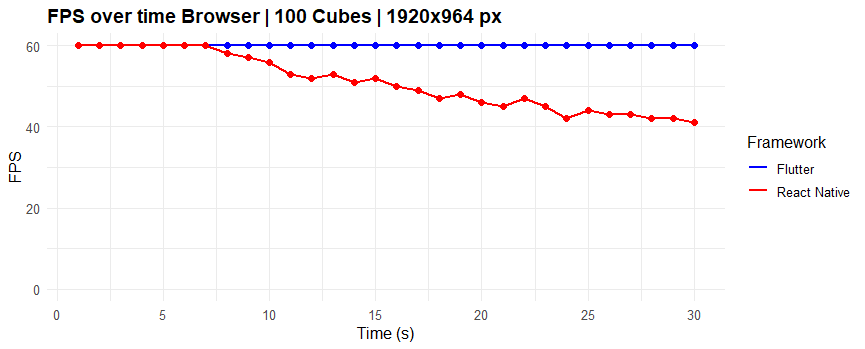
\includegraphics[width=1\linewidth]{images/web/100Cubes.png}
    \caption{FPS über Dauer Web}
\end{figure}

\begin{figure}[H]
    \centering
   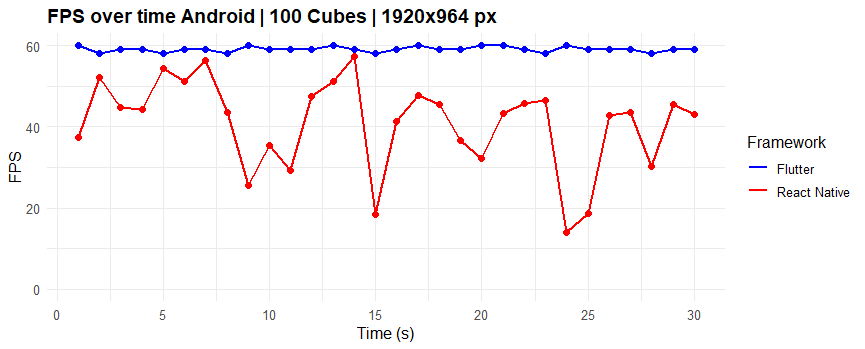
\includegraphics[width=1\linewidth]{images/android/100Cubes.png}
    \caption{FPS über Dauer Android}
\end{figure}

\begin{table}[h!]
    \centering
    \begin{tabular}{llll}
    \toprule
    \textbf{Framework} & \textbf{Plattform} & \textbf{Mittelwert in FPS} & \textbf{Median in FPS} \\
    \midrule
        Flutter & Web & 60 & 60 \\
        Flutter & Android & 59.03 & 59 \\
        React Native & Web & 50.87 & 50.5 \\
        React Native & Android & 40.87 & 43.55 \\
    \bottomrule
    \end{tabular}
\end{table}

Die durchgeführten Tests haben ergeben, dass Flutter in der Lage ist, die Framerate von 60 Bildern pro Sekunde über einen konstanten Zeitraum aufrechtzuerhalten. React Native hingegen hält die 60 FPS bis zur siebten Sekunde stabil, bevor ein langsamer Abfall einsetzt. Auf dem Android-Gerät zeigt Flutter insgesamt eine durchgehend stabile Leistung. Bei der Darstellung von 100 animierten Elementen sind jedoch starke Schwankungen festzustellen, die durch React Native verursacht werden.

Flutter profitiert von seiner plattformunabhängigen Rendering-Engine Skia, die eine direkte und effiziente Darstellung von Animationen ermöglicht. React Native hingegen verwendet den virtuellen DOM und ist von dessen Performance abhängig, wodurch die FPS mit zunehmender Dauer sinken können. Diese Beobachtungen zeigen, dass Flutter in diesem Test performanter ist.

Auf dem Android-Gerät nutzt Flutter ebenfalls seine eigene Rendering-Engine, was zu ähnlichen Ergebnissen wie im Browser führt. React Native muss den JavaScript-Code in die native Sprache übersetzen, was bei vielen Anfragen zu Verzögerungen führt. Allerdings zeigt auch Flutter bei der Darstellung von 100 Würfeln geringfügige Leistungseinbußen.

\newpage
\subsection{1000 Würfel Animation}

\begin{figure}[H]
    \centering
    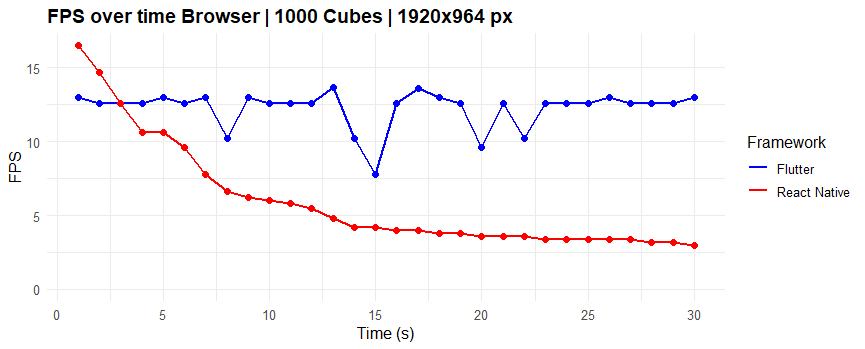
\includegraphics[width=1\linewidth]{images/web/1000Cubes.png}
    \caption{FPS über Dauer Web}
\end{figure}

\begin{figure}[H]
    \centering
    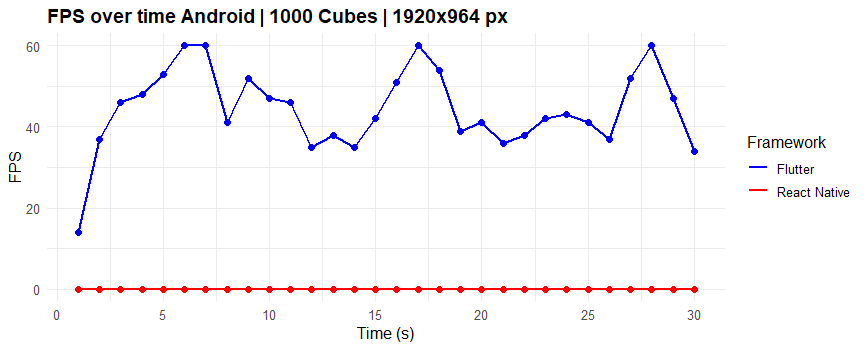
\includegraphics[width=1\linewidth]{images/android/1000Cubes.png}
    \caption{FPS über Dauer Android}
\end{figure}

\begin{table}[h!]
    \centering
    \begin{tabular}{llll}
    \toprule
    \textbf{Framework} & \textbf{Plattform} & \textbf{Mittelwert in FPS} & \textbf{Median in FPS} \\
    \midrule
        Flutter & Web & 12.26 & 12.6 \\
        Flutter & Android & 44.29 & 42.5 \\
        React Native & Web & 5.95 & 4.1 \\
        React Native & Android & 0 & 0 \\
    \bottomrule
    \end{tabular}
\end{table}

Bei 1.000 animierten Würfeln im Browser zeigt Flutter leichte Schwankungen und erzielt FPS im unteren Bereich. React Native erreicht zu Beginn höhere FPS als Flutter, jedoch flacht die Kurve im weiteren Verlauf deutlich ab. Als Android-App zeigt Flutter im Vergleich zur Leistung im Browser eine deutlich bessere Performance. React Native hingegen schafft es bei dieser Anzahl an Elementen nicht, mehr als 0 Bilder pro Sekunde darzustellen.

Mit einer erhöhten Anzahl animierter Elemente erleiden beide Frameworks Leistungseinbußen. Im Browser ist ein geringfügiger Unterschied zu erkennen: Nach einer gewissen Zeit sinkt die Anzahl der Bilder pro Sekunde bei React Native drastisch. Dies ist auf eine Art Stau bei der Manipulation des DOM zurückzuführen.

\newpage
\subsection{Sieb des Erasthenes}
Für diese und folgende Ergebnisse gilt, dass ein niedrigeres Ergebnis eine bessere Leistung darstellt.
\begin{figure}[H]
    \centering
    \includegraphics[width=1\linewidth]{images/web/prime.png}
    \caption{Dauer des Benchmarks im Browser}
\end{figure}

\begin{figure}[H]
    \centering
    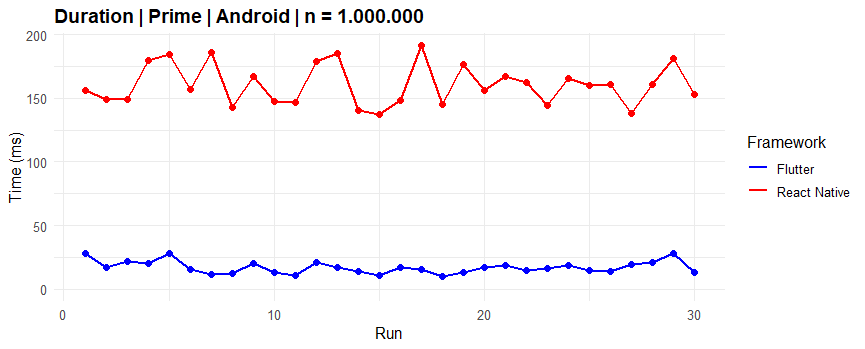
\includegraphics[width=1\linewidth]{images/android/Prime.png}
    \caption{Dauer des Benchmarks im Browser}
\end{figure}

\begin{table}[h!]
    \centering
    \begin{tabular}{llll}
    \toprule
    \textbf{Framework} & \textbf{Plattform} & \textbf{Mittelwert in ms} & \textbf{Median in ms} \\
    \midrule
        Flutter & Web & 4.74 & 4.57 \\
        Flutter & Android & 17.14 & 16.66 \\
        React Native & Web & 7.02 & 6.83 \\
        React Native & Web & 160.72 & 158.61 \\
    \bottomrule
    \end{tabular}
\end{table}

Die in den Abbildungen dargestellten Graphen verdeutlichen, dass auf beiden Plattformen für die Berechnung mit React Native ein höherer Zeitaufwand erforderlich ist. Im Browser zeigen beide Frameworks eine ähnliche Kurve, die einen relativ konstanten Verlauf aufweist.

React Native nutzt für die Berechnung die JavaScript-Engine des Browsers, in diesem Fall V8, während Flutter in der eigenen Dart-VM ausgeführt wird. Der Dart-Code wird mittels AOT-Kompilierung (Ahead-of-Time) direkt auf der Hardware ausgeführt. React Native hingegen führt die Berechnung in der JavaScript-Engine durch, die kontinuierlich einen Interpreter und die JIT-Kompilierung (Just-in-Time) verwendet. Beide Frameworks nutzen JavaScript zur Berechnung der Zahlen, da bei Flutter nur das CanvasKit, welches zur Darstellung von Elementen dient, WebAssembly nutzt.
Die Garbage Collection von Flutter ist speziell auf Dart-Code ausgelegt, was eine inkrementelle und effiziente Speicherverwaltung ermöglicht.

Insgesamt lässt sich feststellen, dass React Native durch verschiedene Eigenschaften wie die dynamische Typisierung, die flexible Array-Verwaltung und die JavaScript-Bridge an Leistung einbüßt.

\newpage
\subsection{State Management}
\begin{figure}[H]
    \centering
    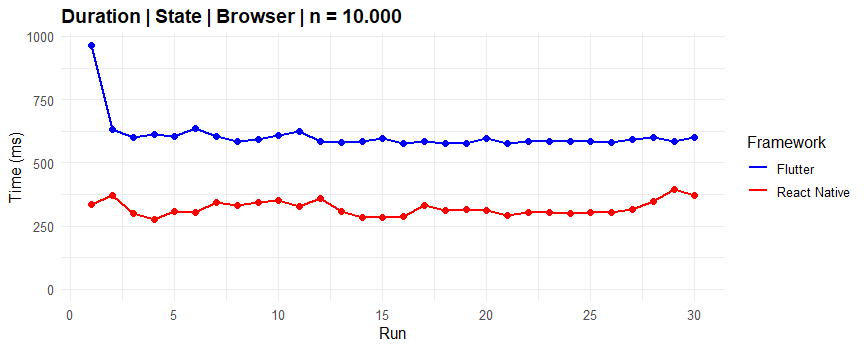
\includegraphics[width=1\linewidth]{images/web/State.png}
    \caption{Dauer des Benchmarks im Browser}
\end{figure}

\begin{figure}[H]
    \centering
    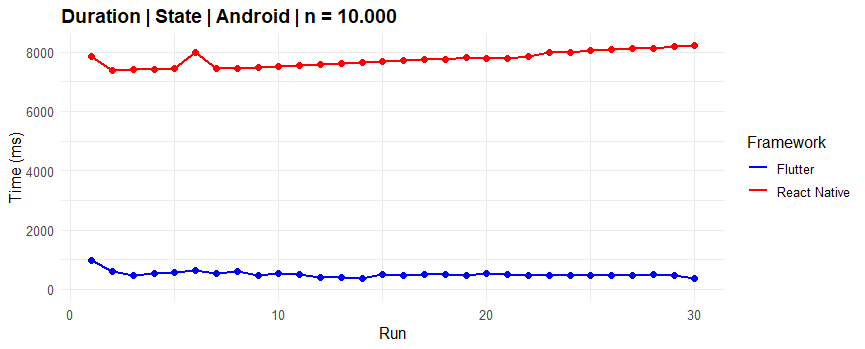
\includegraphics[width=1\linewidth]{images/android/State.png}
    \caption{Dauer des Benchmarks im Browser}
\end{figure}

\begin{table}[h!]
    \centering
    \begin{tabular}{llll}
    \toprule
    \textbf{Framework} & \textbf{Plattform} & \textbf{Mittelwert in ms} & \textbf{Median in ms} \\
    \midrule
        Flutter & Web & 606.13 & 598.67 \\
        Flutter & Android & 506 & 482.16 \\
        React Native & Web & 320.69 & 313 \\
        React Native & Android & 7756.89 & 7762 \\
    \bottomrule
    \end{tabular}
\end{table}

Die Ausführung des Benchmarks erfolgt bei React Native im Browser mit höherer Geschwindigkeit. Beide Graphen zeigen eine konstante Entwicklung, wobei Flutter zu Beginn einen hohen Wert erzielt, der im folgenden Durchlauf deutlich sinkt und danach nahezu konstant bleibt. Als mobile Android-App bleiben die Graphen weiterhin konstant, jedoch erzielt React Native deutlich schlechtere Werte, während Flutter die Messergebnisse verbessert.

Die Geschwindigkeit, mit der Daten in einen State gepackt und wieder daraus gelöscht werden, hängt von der Rendering-Strategie der Frameworks ab. In Flutter Web werden Zustände effizient verarbeitet, jedoch kann der CanvasKit-Renderer bei komplexen Zustandsänderungen zusätzlichen Overhead verursachen, insbesondere bei häufigem UI-Rendering. React Native Web verwendet die JavaScript-Engine des Browsers und aktualisiert das virtuelle DOM, was bei häufigen oder großen Zustandsänderungen zu einer höheren CPU-Belastung führen kann, da das UI bei jeder Änderung neu gerendert wird. Insgesamt kann Flutter bei komplexeren UI-Komponenten langsamer sein, während React Native Web bei häufigen, kleinen Zustandsänderungen aufgrund der virtuellen DOM-Strategie etwas langsamer sein kann.

Auf dem Android-Gerät funktioniert die Kommunikation bei React Native anders: Sämtliche Updates müssen über die Bridge kommuniziert werden. Die Darstellung der Items, die Manipulation der Daten und das Rendern als native Elemente führen zu einer geringeren Leistung. Flutter hingegen ist für mobile Anwendungen optimiert und verwendet Techniken wie AOT-Kompilierung und Widget-Verwaltung, um die Leistung aufrechtzuerhalten.

\newpage
\subsection{Speicher}
\begin{figure}[H]
    \centering
    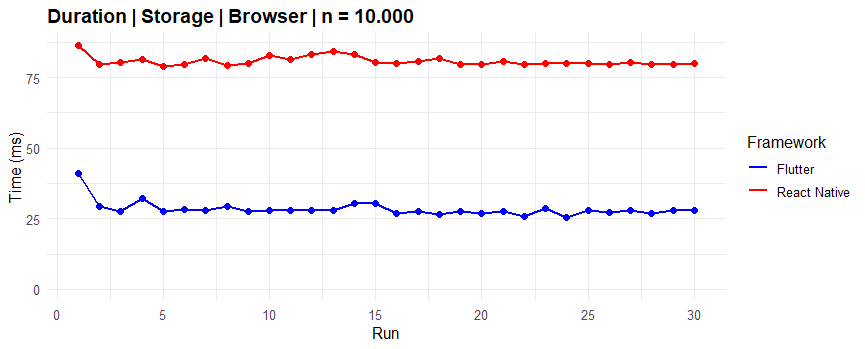
\includegraphics[width=1\linewidth]{images/web/Storage.png}
    \caption{Dauer des Benchmarks im Browser}
\end{figure}

\begin{figure}[H]
    \centering
    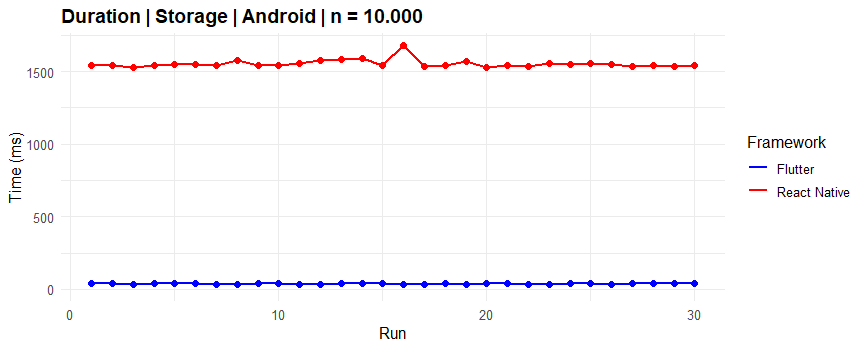
\includegraphics[width=1\linewidth]{images/android/Storage.png}
    \caption{Dauer des Benchmarks im Browser}
\end{figure}

\begin{table}[h!]
    \centering
    \begin{tabular}{llll}
    \toprule
    \textbf{Framework} & \textbf{Plattform} & \textbf{Mittelwert in ms} & \textbf{Median in ms} \\
    \midrule
        Flutter & Web & 28.44 & 28 \\
        Flutter & Android & 37.61 & 37.5 \\
        React Native & Web & 80.82 & 80.09 \\
        React Native & Android & 1553.17 & 1543.83 \\
    \bottomrule
    \end{tabular}
\end{table}


In diesem Test gibt es im Browser bei beiden Frameworks die Gemeinsamkeit, dass sie beide den LocalStorage des Browsers nutzen. React Native Web verwendet ein Polyfill, also eine Bibliothek, die fehlende Funktionen durch alternative Implementierungen bereitstellt, um die Verbindung zum LocalStorage zu ermöglichen. Dies sorgt für Cross-Plattform-Kompatibilität, da derselbe Code sowohl in Web- als auch in nativen Umgebungen funktioniert. Allerdings kann die Verwendung von Polyfills zu Performance-Einbußen führen, da zusätzliche Abstraktionsschichten erforderlich sind, um die Web-API zu emulieren. Flutter Web nutzt ebenfalls JavaScript, um mit Browser-APIs wie LocalStorage zu kommunizieren. Flutter führt den Code nicht direkt auf dem Endgerät aus, sondern transpiliert ihn nach JavaScript, wodurch auch hier keine direkte Kommunikation mit den Web-APIs erfolgt. Daher greifen beide Frameworks auf den LocalStorage zu, allerdings auf unterschiedliche Weise: React Native Web über Polyfills und Flutter Web über JavaScript, ohne Polyfills zu benötigen.

Auf dem Android-Gerät unterscheidet sich die Implementierung der beiden Frameworks. Flutter greift auf die SharedPreferences des Geräts zu, welche für die Speicherung von kleineren Datenmengen optimal sind und zum Großteil synchron sind. React Native nutzt bei der Implementierung eine SQLite-Datenbank, welche die Verwaltung von großen und komplexen Datenmengen verbessert, jedoch für den getesteten Fall einen großen Overhead darstellt. Die Daten werden bei den SharedPreferences als XML-Datei gespeichert, wodurch der Zugriff schnell erfolgt. Bei React Native muss jede Anfrage von Daten über die Datenbank getätigt werden, wodurch es zu Ladezeiten kommt. Das asynchrone Laden von Daten bietet ebenfalls viele Vorteile, hat aber Schwächen bei der Ladezeit.

\newpage

\subsection{Forschungsfragen}
In der Anforderungsanalyse wurde bereits die fundamentale Forschungsfrage mit ihren Unterfragen erwähnt.

\vspace{0.5cm}

\textit{Welche messbaren Unterschiede in der Darstellungsleistung ergeben sich im Vergleich zwischen Flutter und React Native in modernen Cross-Plattform-Anwendungen?}


\begin{enumerate}
    \item Wie unterscheiden sich React Native und Flutter in Render- und Rechenleistung bei typischen Entwicklungsaufgaben?
    \item Gibt es Unterschiede der Leistung auf verschiedenen Endgeräten?
    \item Welches Framework ist für die alltägliche Praxis im Hinblick auf die Leistung attraktiver?
\end{enumerate}


\subsubsection{Beantwortung der Forschungsfrage 1}
Um den quantitativen Unterschied ermitteln zu können, wird die Differenz der Messergebnisse in Abhängigkeit vom Endgerät ermittelt, indem der Mittelwert für den jeweiligen Test von Flutter mit dem Wert von React Native subtrahiert wird.

\begin{table}[h!]
    \centering
    \begin{tabular}{|l|l|p{4cm}|l|}
    \toprule
    \textbf{Benchmark} & \textbf{Platfform} & \textbf{Differenz Flutter React Native}& \textbf{Prozentuale Differenz} \\
    \midrule
    Cube 100   & Web   & 9.13 fps & 17.95 \%       \\
    Cube 100   & Android   & 18.16 fps & 44.43 \%      \\
    Cube 1000  & Web & 6.31 fps & 106.05 \%    \\
    Cube 1000  & Android & 44.29 fps & unendlich \%     \\
    Prime      & Web   & 2.28 ms & 48.12  \%   \\
    Prime      & Android   & 143.58 ms & 838 \%    \\
    State      & Web   & 52.38 ms & 184.05 \%  \\
    State      & Android   & 1515.56 ms & 4033.26 \%   \\
    Storage    & Web   & - 285.44 ms & - 89 \%  \\
    Storage    & Android   & 7250.89 ms & 1434.34 \% \\
    \bottomrule
    \end{tabular}
\end{table}

Die Tabelle zeigt, dass es bei nahezu allen Benchmarks auf allen Endgeräten Leistungsunterschiede gibt, bei denen Flutter die bessere Leistung aufweist. Die einzige Ausnahme ist bei dem Storage Benchmark im Browser, bei dem React Native eine bessere Leistung aufzeigt. Aus diesen Unterschieden lässt sich ableiten, dass Flutter in den getesteten Benchmarks eine bessere Performance im Bereich der Rechen- und Darstellungsleistung aufweist.

\subsubsection{Beantwortung der Forschungsfrage 2}
Die Untersuchung der ersten Forschungsfrage ergab, dass es erhebliche Unterschiede zwischen den einzelnen Frameworks bei der Leistung gibt. Um die Leistungsunterschiede eines Frameworks auf den verschiedenen Geräten zu ermitteln, wird die Differenz der Benchmarks, welche im Browser und auf einem Android-Gerät, berechnet und analysiert. Im Folgenden wird die Differenz der Leistung vom Android-Gerät zum Browser ermittelt und zum Vergleich herangezogen.

\begin{table}[h!]
    \centering
    \begin{tabular}{|l|p{3cm}|p{3cm}|p{3cm}|p{3cm}|}
    \hline
    \textbf{Benchmark} & \textbf{Differenz (Flutter)} & \textbf{Prozentual Flutter} & \textbf{Differenz (React Native)} & \textbf{Prozentual React Native} \\
    \hline
    Cube 100   & 0.97 fps & 1.64 \% & 10 fps & 24.4 \% \\
    Cube 1000  & -32.03 fps & -261.16 \% & 5.95 fps & unendlich \% \\
    Prime      & 12.4 ms & 261.18 \% & 153.7 ms & 2191.56 \% \\
    State      & -100 ms & -19.7 \% & 7436.2 ms & 2320.35 \% \\
    Storage    & 9.71 ms & 32.2 \% & 1472.35 ms & 1822.27 \% \\
    \hline
    \end{tabular}
    \caption{Vergleich der Differenzen und prozentualen Unterschiede zwischen Flutter und React Native Benchmarks}
\end{table}


Anhand der Tabelle lässt sich erkennen, dass es bei React Native in allen Benchmarks zu Ergebnissen kommt, welche belegen, dass die Leistung von React Native auf dem Android-Gerät konstant schlechter ist, als im Browser. Die signifikante Diskrepanz der ermittelten Mittelwerte in Bezug auf React Native lässt die Vermutung zu, dass die Leistung von React Native auf unterschiedlichen Endgeräten erheblich variiert.

Die Auswertungen der Differenzen von Flutter zeigen, dass bei zwei Benchmarks eine bessere Performance auf dem Android-Gerät im Vergleich zum Browser vorliegt. Die sich daraus ergebenden Unterschiede bewegen sich in einem geringen Bereich von maximal 100 Millisekunden bei den Leistungstests. Bei der Darstellung der Würfel gibt es bei einer hohen Anzahl von Würfeln einen Unterschied von bis zu 30 Frames pro Sekunde auf dem Android-Gerät. In der Praxis unter realistischen Bedingungen stellen die Leistungstests keinen merkbaren Unterschied dar. Die Analyse der vorliegenden Daten ergibt, dass die Darstellung und Animation einer hohen Anzahl von Elementen, die 100 nicht überschreitet, keinen signifikanten Unterschied aufweist.

\subsubsection{Beantwortung der Forschungsfrage 3}
Die Benchmarks dieser Arbeit nutzten teilweise für die Praxis unrealistische Bedingungen. Hierzu zählt die große Anzahl an animierten Elementen, sehr häufiges Wechseln des Zustands oder eine Speicherung von unzähligen Daten auf dem Endgerät. Realitätsnähere Werte sorgen für eine geringere Diskrepanz im Vergleich der beiden Frameworks. Dies wurde in einem kleinen Ausschnitt getestet, indem das n der jeweiligen Benchmarks drastisch reduziert und die Ergebnisse in einer Tabelle festgehalten wurden. Es wurden 30 Messungen durchgeführt und die Mittelwerte der Messungen zum Vergleich herangezogen.

\begin{table}[h!]
    \centering
    \begin{tabular}{|l|l|p{3cm}|p{3cm}|p{4cm}|}
    \toprule
    \textbf{Benchmark} & \textbf{Platfform}  & \textbf{Differenz Flutter React Native} & \textbf{Prozentuale Differenz} & \textbf{Mittelwerte Flutter / React Native} \\
    \midrule
    Cube | n = 5   & Web   & 0 fps & 0 \%  & 60 / 60 fps     \\
    Cube | n = 5   & Android   & 0 fps & 0 \% & 60 / 60 fps    \\
    Prime | n = 100      & Web   & 1.467 ms & unendlich \% & 0 / 1.467 ms   \\
    Prime | n = 100      & Android   & 13.961 ms & 305,6 \% & 4.567 / 18.528 ms    \\
    State | n = 10      & Web   & 4.003 ms & 7,76 \% & 52 / 56.033 ms  \\
    State | n = 10      & Android   & 24.788 ms & 47,8 \% & 51.867 / 76.655 ms   \\
    Storage | n = 10    & Web   & 0.003 ms & 1,80 \% & 0.167 / 0.170 ms \\
    Storage | n = 10    & Android   & 2.137 ms & 12,99 \% & 15.767 / 17.815 ms \\
    \bottomrule
    \end{tabular}
\end{table}

Die Tabelle zeigt, dass es nur geringfügige Unterschiede bei den Ergebnissen gibt, welche mit einem kleineren n ermittelt wurden. Eine Differenz von wenigen Millisekunden wird in der Praxis keinen Einfluss auf das Nutzererlebnis haben. Eine Empfehlung für die alltägliche Praxis anhand der Messergebnisse lässt sich bedingt aufstellen, jedoch ist Flutter im Bereich der Leistung ein Stück voraus.

\subsubsection{Beantwortung der fundamentalen Forschungsfrage}
Die fundamentale Forschungsfrage untersucht die messbaren Unterschiede in der Darstellungsleistung zwischen Flutter und React Native in modernen Cross-Plattform-Anwendungen. Die Ergebnisse der Teilfragen zeigen, dass Flutter in den meisten getesteten Benchmarks hinsichtlich der Render- und Rechenleistung überlegen ist. In der ersten Teilfrage wurde deutlich, dass Flutter in nahezu allen Kategorien, wie etwa bei der Darstellung von Würfeln und der Berechnung von Primzahlen, eine bessere Performance bietet. Die einzige Ausnahme bildet der Storage-Benchmark im Browser, bei dem React Native besser abschneidet. In der zweiten Teilfrage wurde festgestellt, dass React Native auf verschiedenen Endgeräten, insbesondere auf Android, eine schlechtere Leistung zeigt als im Browser, während die Leistungsunterschiede von Flutter zwischen den Geräten deutlich geringer ausfallen. In der dritten Teilfrage wurde darauf hingewiesen, dass die getesteten Benchmarks unter teilweise unrealistischen Bedingungen durchgeführt wurden. Unter realistischeren Nutzungsszenarien zeigt Flutter jedoch weiterhin eine bessere Performance. Zusammenfassend lässt sich sagen, dass Flutter im Bereich der Darstellungsleistung und Rechenleistung insgesamt die bessere Wahl ist, insbesondere bei anspruchsvolleren Anwendungen, bei denen Leistung eine entscheidende Rolle spielt.
\section{Exkurs}
\subsection{Anpassung der Frameworks}
Beide Frameworks befinden sich zudem in ständiger Weiterentwicklung. So wurde bei React Native die Bridge, die bisher die Kommunikation zwischen JavaScript und der nativen Plattform verwaltet hat, durch die neue Fabric-Architektur ersetzt \cite{ReactNativeNewArchitecture}. Dies führt zu einer effizienteren und direkteren Ausführung nativer Module. Diese Änderungen sowie weitere Optimierungen, wie etwa ein gezieltes State-Management oder die Wahl effizienter Speicherlösungen, können signifikanten Einfluss auf die Performance haben.

\vspace{0.5cm}

Dazu gehört beispielsweise die Möglichkeit, Skia \cite{ReactNativeSkia} als Rendering-Engine in React Native zu integrieren oder eine andere Technik zu verwenden, um den Zustand in Flutter granular und performant zu gestalten \cite{FlutterBloc}.

\vspace{0.5cm}

Die verwendeten Bibliotheken sind nicht maßgeblich die effizientesten für die getesteten Anwendungsfälle. Es wurden Bibliotheken verwendet, die sehr häufig in der Entwicklung mit den jeweiligen Frameworks verwendet wurden oder von den Entwicklern empfohlen wurden.

\subsection{Unterschiede im Design}
Ein weiterer nicht messbarer Punkt der beiden Frameworks ist die Darstellung im UI. Hierbei gibt es gravierende Unterschiede, denn React Native ist in der Lage die nativen Komponenten des Endgeräts darzustellen. Dies ermöglicht mit einer einheitlichen Codegrundlage, dass die App auf einem Android-Gerät optisch sich stark unterscheidet im Vergleich zum iOS-Gerät. Flutter nutzt ein eigenes Design und bildet dieses auf allen Endgeräten ab. Im Anhang habe ich ein Formular entwickelt, welches einen Teil der essenziellen Elemente darstellt und auf verschiedenen Endgeräten getestet.
,\section{Fazit}
Die Ergebnisse dieser Arbeit zeigen, dass sowohl Flutter als auch React Native ihre spezifischen Stärken und Schwächen haben, die von der jeweiligen Anwendung und den Einsatzbedingungen abhängen. Flutter zeichnet sich in den meisten Benchmarks durch eine bessere Performance aus, insbesondere bei grafikintensiven Aufgaben und der Animation einer großen Anzahl von Elementen. Dies liegt vor allem an der nativen Rendering-Engine Skia, die eine direkte Kontrolle über die Darstellung der UI bietet. React Native hingegen ist durch die JavaScript-Bridge limitiert, die in komplexen Szenarien zu Leistungseinbußen führt.

Im Bereich des State Managements zeigt Flutter durch seine AOT-Kompilierung und das effiziente Widget-System eine stabilere Leistung, während React Native durch die Bridge-Architektur auf mobilen Geräten Schwierigkeiten hat. Beim Speichern und Verarbeiten von Daten hat Flutter ebenfalls Vorteile, da es auf plattformspezifische Optimierungen wie SharedPreferences setzt. React Native kann in einigen Szenarien im Web konkurrenzfähig bleiben, jedoch treten auf mobilen Plattformen deutliche Schwächen auf.

Die Untersuchung hat zudem gezeigt, dass die Wahl der Frameworks stark von den spezifischen Anforderungen eines Projekts abhängt. Während Flutter durch seine hohe Performance und plattformübergreifende Konsistenz punktet, bietet React Native eine größere Flexibilität bei der Integration nativer Funktionen und eine stärkere Anpassung an das Design der Zielplattformen.

Zukünftige Entwicklungen könnten diese Unterschiede weiter beeinflussen. So könnten die neue Fabric-Architektur in React Native und die Integration von Skia als Rendering-Engine erhebliche Performance-Verbesserungen bringen. Auch Flutter bleibt durch kontinuierliche Optimierungen ein leistungsstarkes Framework für moderne Cross-Plattform-Anwendungen.

Abschließend lässt sich festhalten, dass Flutter derzeit bei den getesteten Benchmarks die bessere Performance bietet, während React Native durch seine Vielseitigkeit und größere Community besticht. Eine eindeutige Empfehlung, welches Framework in der täglichen Praxis zu empfehlen ist, kann jedoch nicht gegeben werden, da dies von vielen Faktoren abhängt. Dazu gehören die Erfahrung der Entwickler, die persönliche Präferenz und der Anwendungsfall. Die praxisnahen Messungen haben jedoch gezeigt, dass die Frameworks im Alltag eine nahezu identische Performance erzielen.
\section*{Anhang}
\addcontentsline{toc}{section}{Anhang}
\begin{figure}[H]
    \centering
    \textbf{Darstellung des Formulars mit Flutter Android}\par\vspace{0.5cm}
    \begin{minipage}{0.45\textwidth}
        \centering
        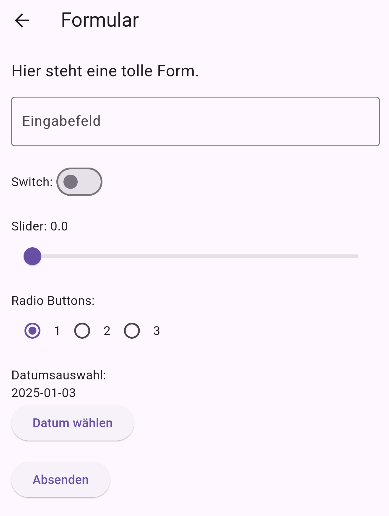
\includegraphics[width=\linewidth]{images/form/android/flutter/form.png}
        \caption{Unausgefülltes Formular Flutter Android}
    \end{minipage}
    \hfill
    \begin{minipage}{0.45\textwidth}
        \centering
        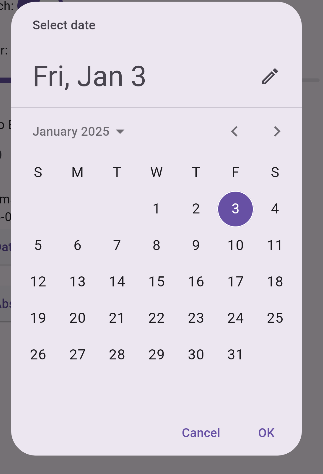
\includegraphics[width=\linewidth]{images/form/android/flutter/dateOpen.png}
        \caption{Date Picker Flutter Android}
    \end{minipage}

    \vspace{0.5cm}

    \begin{minipage}{0.45\textwidth}
        \centering
        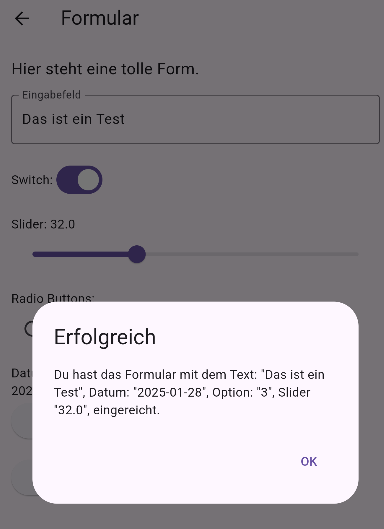
\includegraphics[width=\linewidth]{images/form/android/flutter/modal.png}
        \caption{Modal Flutter Android}
    \end{minipage}
    \hfill
    \begin{minipage}{0.45\textwidth}
        \centering
        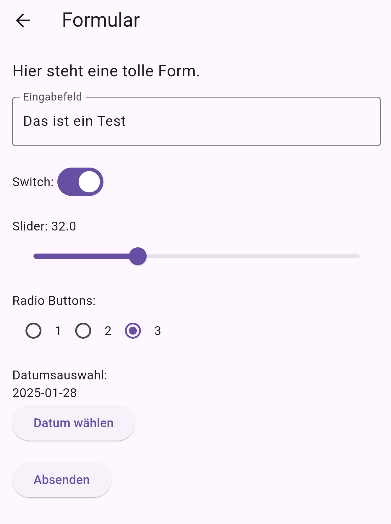
\includegraphics[width=\linewidth]{images/form/android/flutter/formCompleted.png}
        \caption{Ausgefüllt Formular Flutter Android}
    \end{minipage}
\end{figure}

\begin{figure}[H]
    \centering
    \textbf{Darstellung des Formulars mit React Native Android}\par\vspace{0.5cm}
    \begin{minipage}{0.45\textwidth}
        \centering
        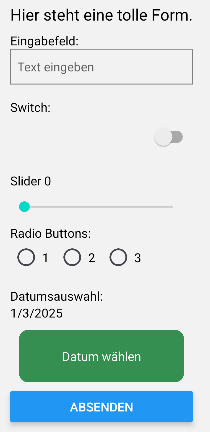
\includegraphics[width=\linewidth]{images/form/android/react_native/form.png}
        \caption{Unausgefülltes Formular React Native Android}
    \end{minipage}
    \hfill
    \begin{minipage}{0.45\textwidth}
        \centering
        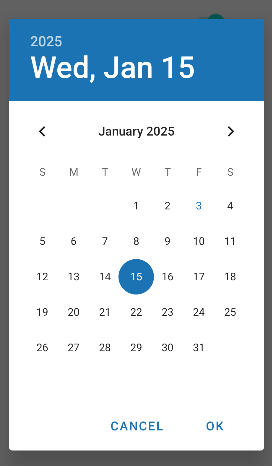
\includegraphics[width=\linewidth]{images/form/android/react_native/dateOpen.png}
        \caption{Date Picker React Native Android}
    \end{minipage}

    \vspace{0.5cm}

    \begin{minipage}{0.45\textwidth}
        \centering
        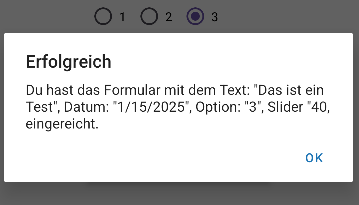
\includegraphics[width=\linewidth]{images/form/android/react_native/modal.png}
        \caption{Modal React Native Android}
    \end{minipage}
    \hfill
    \begin{minipage}{0.45\textwidth}
        \centering
        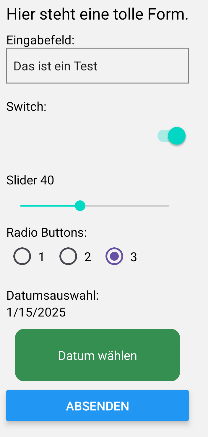
\includegraphics[width=\linewidth]{images/form/android/react_native/formCompleted.png}
        \caption{Ausgefüllt Formular React Native Android}
    \end{minipage}
\end{figure}

\begin{figure}[H]
    \centering
    \textbf{Darstellung des Formulars mit Flutter Web}\par\vspace{0.5cm}
    \begin{minipage}{0.45\textwidth}
        \centering
        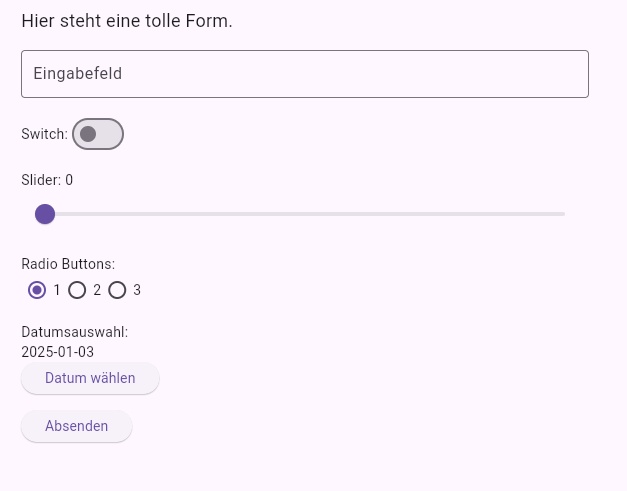
\includegraphics[width=\linewidth]{images/form/web/flutter/form.png}
        \caption{Unausgefülltes Formular Flutter Web}
    \end{minipage}
    \hfill
    \begin{minipage}{0.45\textwidth}
        \centering
        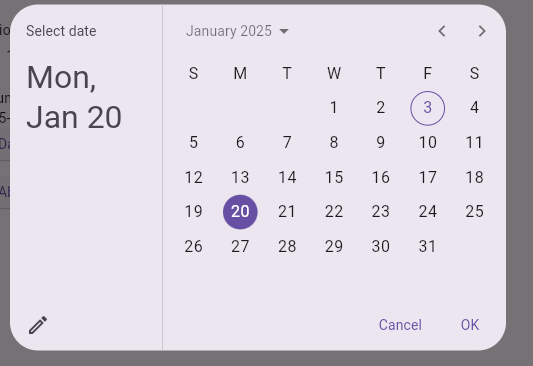
\includegraphics[width=\linewidth]{images/form/web/flutter/dateOpen.png}
        \caption{Date Picker Flutter Web}
    \end{minipage}

    \vspace{0.5cm}

    \begin{minipage}{0.45\textwidth}
        \centering
        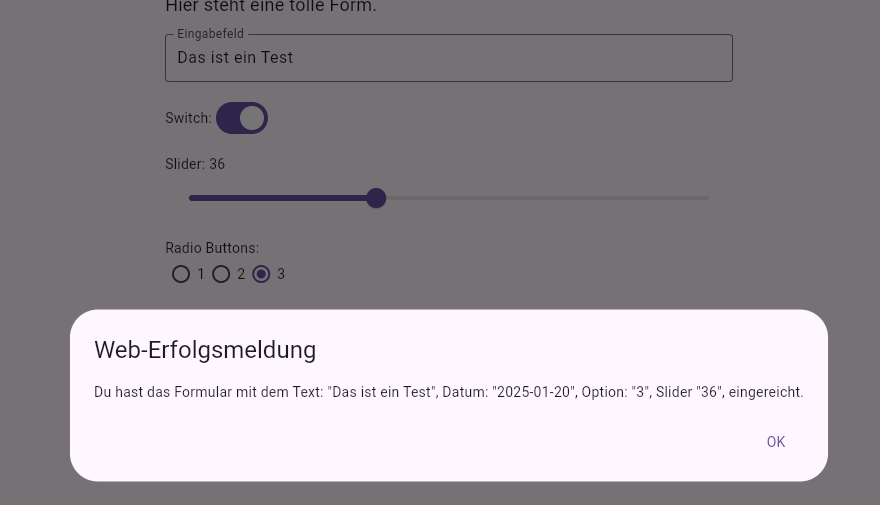
\includegraphics[width=\linewidth]{images/form/web/flutter/modal.png}
        \caption{Modal Flutter Web}
    \end{minipage}
    \hfill
    \begin{minipage}{0.45\textwidth}
        \centering
        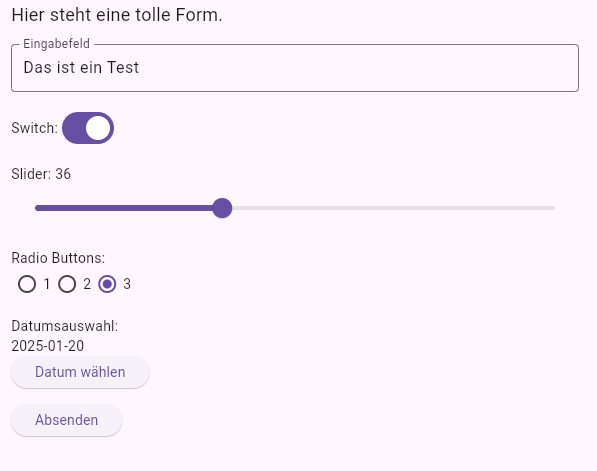
\includegraphics[width=\linewidth]{images/form/web/flutter/formCompleted.png}
        \caption{Ausgefüllt Formular Flutter Web}
    \end{minipage}
\end{figure}

\begin{figure}[H]
    \centering
    \textbf{Darstellung des Formulars mit React Native Web}\par\vspace{0.5cm}
    \begin{minipage}{0.45\textwidth}
        \centering
        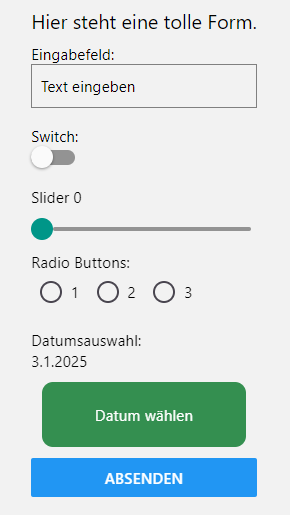
\includegraphics[width=\linewidth]{images/form/web/react_native/form.png}
        \caption{Unausgefülltes Formular React Native Web}
    \end{minipage}
    \hfill
    \begin{minipage}{0.45\textwidth}
        \centering
        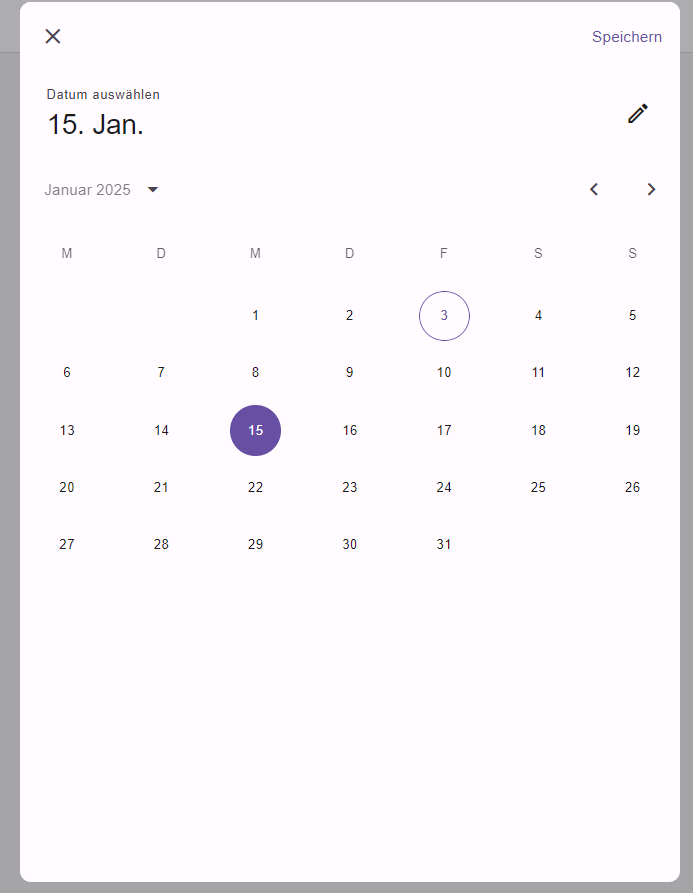
\includegraphics[width=\linewidth]{images/form/web/react_native/dateOpen.png}
        \caption{Date Picker React Native Web}
    \end{minipage}

    \vspace{0.5cm}

    \begin{minipage}{0.45\textwidth}
        \centering
        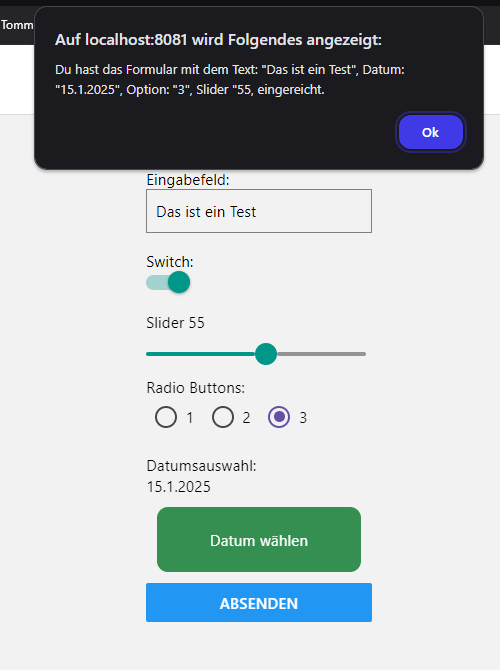
\includegraphics[width=\linewidth]{images/form/web/react_native/modal.png}
        \caption{Modal React Native Web}
    \end{minipage}
    \hfill
    \begin{minipage}{0.45\textwidth}
        \centering
        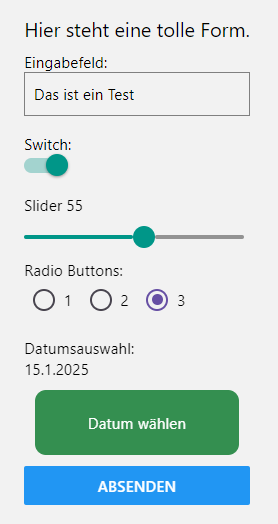
\includegraphics[width=\linewidth]{images/form/web/react_native/formCompleted.png}
        \caption{Ausgefüllt Formular React Native Web}
    \end{minipage}
\end{figure}

\nocite{*}
\printbibliography[notkeyword=Quelle,title={Literaturverzeichnis},heading=subbibliography]


\end{document}
